\documentclass{article}
\usepackage{fontspec}
\usepackage{graphicx}
\usepackage{fancyhdr}
\usepackage{geometry}
\usepackage{lipsum}
\usepackage[spanish]{babel}
\usepackage{xcolor}
\usepackage{eso-pic}
\usepackage{tikz}
\usepackage{atbegshi}
\usepackage[most]{tcolorbox} 
\usepackage{listings}
\usepackage{fontawesome5}

\usetikzlibrary{backgrounds}

\setmainfont[
    Path = ./fonts/Poppins/,
    Extension = .ttf,
    UprightFont = *-Regular.ttf,
    BoldFont = *-Bold.ttf,
    ItalicFont = *-Italic.ttf,
    BoldItalicFont = *-BoldItalic.ttf,
    % LetterSpace=5, 
]{Poppins}



\newlength{\borderwidth}
\setlength{\borderwidth}{20pt} 


\geometry{a4paper,
          left=\dimexpr1cm+\borderwidth,
          right=\dimexpr1cm+\borderwidth,
          top=\dimexpr2cm+\borderwidth,
          bottom=\dimexpr0.5cm+\borderwidth,
          headheight=1.5cm,
          headsep=0.5cm}


\pagestyle{fancy}
\fancyhf{}
\fancyhead[L]{\raisebox{0\height}{
\includegraphics[height=1cm,keepaspectratio]{logo-header.png}}}
\fancyhead[R]{\raisebox{1.25\height}{\large\textbf{Academia Juvenil de Programación Competitiva}}}
\renewcommand{\headrulewidth}{0pt}


\definecolor{primary}{HTML}{116BB1}
\definecolor{secondary}{HTML}{711E8C}
\definecolor{tertiary}{HTML}{1ECA6C}


\newcommand{\borderOverlay}{
    \begin{tikzpicture}[remember picture, overlay]
        \draw[line width=\borderwidth, color=primary]
            (current page.north west) -- 
            (current page.north east) --
            (current page.south east) --
            (current page.south west) -- cycle;
    \end{tikzpicture}
}

\AddToShipoutPictureBG{\borderOverlay}

\newtcolorbox{container}[1]{ 
    colback=white, 
    colframe=primary,
    coltitle=white,
    title={#1},
    fonttitle=\bfseries, 
    arc=2pt,
    boxrule=2pt, 
    enhanced, 
    breakable, 
    attach boxed title to top left={xshift=5pt, yshift=-5pt}, 
    boxed title style={colback=primary, size=small}, 
}


\lstdefinestyle{cppstyle}{
    language=C++,
    basicstyle=\ttfamily\small,
    keywordstyle=\color{primary},
    commentstyle=\color{tertiary},
    stringstyle=\color{secondary},
    backgroundcolor=\color{white!100},
    breaklines=true,
    breakatwhitespace=true,
    tabsize=4,
    showstringspaces=false,
    captionpos=b
}

\newcommand{\cppfile}[2][]{
    \begin{container}{\faCode \space \space  #1}
        \lstinputlisting[style=cppstyle]{#2}
    \end{container}
}

\newcommand{\inlinecpp}[1]{
    \lstinline[
        language=C++,
        basicstyle=\ttfamily\small\color{primary!80!black},
        keywordstyle=\color{primary},
        stringstyle=\color{secondary},
        commentstyle=\color{tertiary}
    ]|#1|
}


\newcommand{\documentTitle}{Clase 4}
\newcommand{\documentSubtitle}{Contenidos y ejercicios prácticos}
\newcommand{\documentAuthor}{Francisco Muñoz}
\newcommand{\documentDate}{16 de Agosto}

\begin{document}

\thispagestyle{empty}
\AddToShipoutPictureBG*{}
\begin{center}
    \vspace*{2cm}
    
\includegraphics[width=0.75\textwidth]{logo.png} \\[1.5cm]
    {\Huge \textbf{\documentTitle}} \\[0.5cm]
    {\Large \documentSubtitle} \\[1.5cm]
    {\large \documentAuthor} \\[0.5cm]
    {\large \space \space \documentDate}
    \vfill
    {\large Academia Juvenil de Programación Competitiva}
\end{center}
\newpage

\section{Introducción}

En esta clase aprenderemos un concepto fundamental en la programación: los \textbf{bucles}.
Un bucle es una estructura que nos permite repetir un bloque de código varias veces sin tener que escribirlo repetidamente.

\section{Índice}

\begin{itemize}
    \item Contenidos
    \begin{itemize}
        \item Bucles: Ejemplo motivador
        \item ¿Qué es un bucle?
        \item Tipos de bucles en C++
    \end{itemize}
    \item Ejercicios Prácticos
\end{itemize}

\section{Contenidos}

\subsection{Ejemplo motivador}

Imagina que quieres mostrar en pantalla los números del 1 al 10. Según todo lo visto hasta ahora, esto podría realizarse de la siguiente manera:

\cppfile[Sin bucles]{codes/nobucle.cpp}

Esto funciona, pero es poco práctico, repetitivo y propenso a errores. Con bucle podemos lograr lo mismo con mucho menos código.

\cppfile[Con bucles]{codes/conbucle.cpp}


\subsection{¿Qué es un bucle?}

Un bucle es una estructura de control que permite ejecutar un conjunto de instrucciones repetidamente mientras se cumpla una condición o hasta que se alcance un objetivo.


\textbf{Ventaja de usar bucles:}

\begin{itemize}
    \item Reducen la cantidad de código repetitivo.
    
    \item Facilitan cambios: si queremos llegar hasta 100 en vez de 10, solo cambiamos un número.

    \item Hacen el código más ordenado y fácil de leer.
\end{itemize}

\vspace{0.5cm}

\section{Tipos de bucles en C++}

\subsection{\texttt{for}}

El bucle \texttt{for} se utiliza cuando sabemos de antemano cuántas veces queremos que se repita el bloque de código.

\textbf{Estructura básica:}

\cppfile[Sintaxis]{codes/buclefor1.cpp}
% \begin{center}
    % 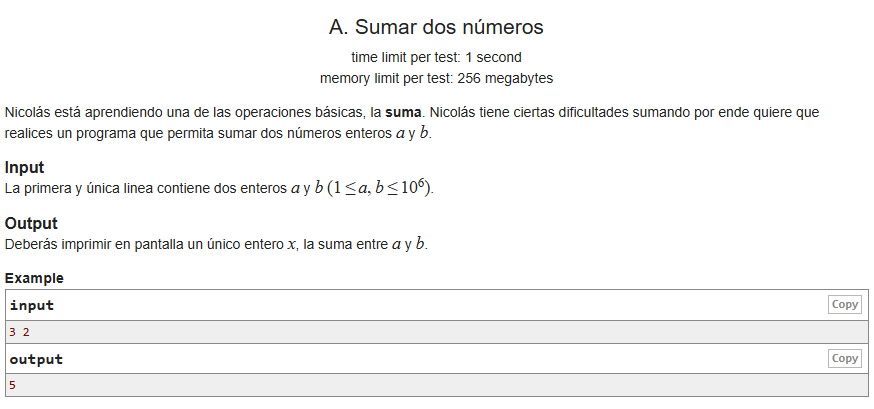
\includegraphics[width=0.8\textwidth]{img/statementexample.png}
    % 
    % \textit{Ejemplo de problema con estructura clásica.}
% \end{center}

\textbf{Partes del for:}
\begin{itemize}
    \item \textbf{Inicialización:} Se ejecuta una vez al inicio, normalmente para declarar y dar valor inicial a la variable de control.
    \item \textbf{Condición:} Se evalúa antes de cada iteración. Si es verdadera, se ejecuta el bloque; si es falsa, el bucle termina.
    \item \textbf{Actualización:} Se ejecuta al final de cada iteración para cambiar el valor de la variable de control.
        Ejemplo: \texttt{i++}
\end{itemize}


\cppfile[Ejemplo de for]{codes/ejemplofor.cpp}

\vspace{0.5cm}

\subsection{\texttt{while}}

El bucle \texttt{while} se utiliza cuando no sabemos exactamente cuántas veces se repetirá el código, pero sí sabemos la condición que debe cumplirse para continuar.

\textbf{Estructura básica:}
\cppfile[Sintaxis]{codes/buclewhile1.cpp}

El \texttt{while} evalúa la condición antes de ejecutar el bloque. Si es verdadera, se ejecuta el bloque; si es falsa, el bucle se detiene.

\textbf{Ejemplo}
\cppfile[Ejemplo de While]{codes/while.cpp}
\section{Ejercicios Prácticos}

\begin{container}{Problema 1 – Contando hasta N}
Escribe un programa que reciba un entero positivo $N$ e imprima los números del 1 al $N$, cada uno en una línea.
\end{container}

\textbf{Input}

Un número entero $N$ ($1 \leq N \leq 100$).

\vspace{0.5em}
\textbf{Output}

Los números del 1 al $N$, cada uno en una línea.

\vspace{0.5em}

\begin{container}{Ejemplo - Input}
5
\end{container}

\begin{container}{Ejemplo - Output}
1\\
2\\
3\\
4\\
5
\end{container}

\vspace{3.5em}


\begin{container}{Problema 2 – Suma de los primeros N números}
Escribe un programa que reciba un entero positivo $N$ y calcule la suma de los números del 1 al $N$.
\end{container}

\textbf{Input}

Un número entero $N$ ($1 \leq N \leq 1000$).

\vspace{0.5em}
\textbf{Output}

Un único número: la suma de $1 + 2 + \dots + N$.

\vspace{0.5em}

\begin{container}{Ejemplo - Input}
4
\end{container}

\begin{container}{Ejemplo - Output}
10
\end{container}

\vspace{3.5em}


\begin{container}{Problema 3 – Tabla de multiplicar}
Escribe un programa que reciba un entero $N$ y muestre su tabla de multiplicar desde $1 \times N$ hasta $10 \times N$.
\end{container}

\textbf{Input}

Un número entero $N$ ($1 \leq N \leq 20$).

\vspace{0.5em}
\textbf{Output}

Diez líneas con la tabla de multiplicar de $N$.

\vspace{0.5em}

\begin{container}{Ejemplo - Input}
3
\end{container}

\begin{container}{Ejemplo - Output}
3\\
6\\
9\\
12\\
15\\
18\\
21\\
24\\
27\\
30
\end{container}

\vspace{3.5em}


\begin{container}{Problema 4 – Contador regresivo}
Escribe un programa que reciba un número entero positivo $N$ y muestre los números desde $N$ hasta $1$, en orden descendente.
\end{container}

\textbf{Input}

Un número entero $N$ ($1 \leq N \leq 100$).

\vspace{0.5em}
\textbf{Output}

Los números desde $N$ hasta $1$, cada uno en una línea.

\vspace{0.5em}

\begin{container}{Ejemplo - Input}
5
\end{container}

\begin{container}{Ejemplo - Output}
5\\
4\\
3\\
2\\
1
\end{container}

\vspace{3.5em}


\begin{container}{Problema 5 – Suma de números positivos}
Escribe un programa que lea una secuencia de enteros y calcule la suma solo de los números positivos. El programa termina cuando se ingrese el número $0$.
\end{container}

\textbf{Input}

Una secuencia de números enteros (pueden ser positivos o negativos). Termina con un $0$.

\vspace{0.5em}
\textbf{Output}

Un único entero: la suma de todos los números positivos ingresados.

\vspace{0.5em}

\begin{container}{Ejemplo - Input}
5 3 -2 4 -1 0
\end{container}

\begin{container}{Ejemplo - Output}
12
\end{container}



\end{document}